\begin{frame}
  \frametitle{Discontinuous Galerkin: notation}

  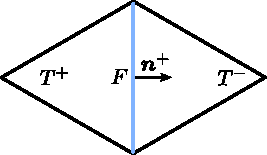
\includegraphics[scale=1.0]{pdf/dg-terms-interface.pdf}

  \begin{columns}[t]
    \begin{column}{0.5\textwidth}
      \alert{Average of a scalar field}: \\ $\avg{v} = \tfrac{1}{2} (v^+ + v^-)$ \\
      \bigskip

      \alert{Jump of a scalar field}: \\ $\jump{v} = (v^+ - v^-) n$
    \end{column}
    \begin{column}{0.5\textwidth}
      \alert{Average of a vector field}: \\ $\avg{B} = \tfrac{1}{2} (B^+ + B^-)$ \\
      \bigskip
      \alert{Jump of a vector field}: \\ $\jump{B} = (B^+ - B^-) \cdot n$
    \end{column}
  \end{columns}

  \bigskip

  {\alert{Jump identity} (Exercise for the reader!)}
  \begin{equation*}
    \jump{B v } = \jump{B} \avg{v}
    + \avg{B} \jump{v}
  \end{equation*}
\end{frame}
